\documentclass[handout]{beamer}
\usepackage{amsmath,amssymb,amsthm,array}
\usepackage{bm}
\usepackage{multirow}
\usepackage{multicol}
\usepackage{algorithm}
\usepackage{hyperref}
\usepackage{algorithmic}
\usepackage[normalem]{ulem}
\usepackage{fontspec}
\usepackage{numprint}

\setmainfont{CMU Serif}
\setsansfont{CMU Sans Serif}
\newfontfamily{\greekfont}{CMU Serif}
\newfontfamily{\greekfontsf}{CMU Sans Serif}
\usetheme{Rochester}
\usecolortheme{crane}

\setbeamertemplate{navigation symbols}{}
\title{Αποδείξεις Μηδενικής Γνώσης}
\author{Παναγιώτης Γροντάς}
\date{16/12/2016}
\defbeamertemplate*{footline}{shadow theme}
{%
  \leavevmode%
  \hbox{\begin{beamercolorbox}[wd=.5\paperwidth,ht=2.5ex,dp=1.125ex,leftskip=.3cm plus1fil,rightskip=.3cm]{author in head/foot}%
    \usebeamerfont{author in head/foot}\insertframenumber\,/\,\inserttotalframenumber\hfill  (\insertshortinstitute)
  \end{beamercolorbox}%
  \begin{beamercolorbox}[wd=.5\paperwidth,ht=2.5ex,dp=1.125ex,leftskip=.3cm,rightskip=.3cm plus1fil]{title in head/foot}%
    \usebeamerfont{title in head/foot}\insertshorttitle%
  \end{beamercolorbox}}%
  \vskip0pt%
}
\institute{ΕΜΠ - Κρυπτογραφία (2016-2017)}
 
 \hypersetup{
  pdfauthor={Panagiotis Grontas},
  pdftitle={Zero Knowledge Proofs},
  colorlinks=true,
  urlcolor=blue,
  linkcolor=white
}

\setlength{\columnseprule}{0.4pt}
\begin{document}
\newcommand{\xor}{ \oplus }
\newcommand{\msg}{ \mathtt{M} }
\newcommand{\KEY}{ \mathtt{K} }
\newcommand{\prv}{$\mathcal{P}$ }
\newcommand{\ver}{$\mathcal{V}$ }
\newcommand{\siml}{$\mathcal{S}$ }
\newcommand{\CPH}{ \mathtt{C} }
\newcommand{\keygen}{\mathtt{KeyGen}}
\newcommand{\enc}{\mathtt{Encrypt}}
\newcommand{\dec}{\mathtt{Decrypt}}
\newcommand{\sign}{\mathtt{Sign}}
\newcommand{\verify}{\mathtt{Verify}}
\newcommand{\adv}{$\mathcal{A}$}
\newcommand{\Hash}{\mathcal{H}}
\newcommand{\advb}{$\mathcal{B}$}
\newcommand{\chal}{$\mathcal{C}$}
\newcommand{\cs}{$\mathcal{CS}$}
\newcommand{\Zed}{\mathbb{Z}} 
\newcommand{\zns}{\mathbb{Z}^*_n}
\newcommand{\zs}[1]{\mathbb{Z}^*_{#1}}

\newcommand{\green}[1]{\textcolor{teal}{#1}}
\newcommand{\Green}[1]{\textcolor{Teal}{#1}}
\newcommand{\ForestGreen}[1]{\textcolor{ForestGreen}{#1}}
\newcommand{\blue}[1]{\textcolor{blue}{#1}}
\newcommand{\magenta}[1]{\textcolor{magenta}{#1}}
\newcommand{\cyan}[1]{\textcolor{cyan}{#1}}

\newcommand{\twopartdef}[4]
{ 
		\begin{cases}
			#1 , #2 \\
			#3 , #4
		\end{cases} 
}
\begin{frame}
\titlepage
\end{frame}

\begin{frame}{Περιεχόμενα}
\begin{itemize}
\item Εισαγωγή
\pause
\item Ορισμός - Εφαρμογές στην Θ. Πολυπλοκότητας
\pause
\item Σ-πρωτόκολλα
\pause
\item Πρακτικές Παραλλαγές και Εφαρμογές
\end{itemize}
\end{frame}

\section{Εισαγωγή}
\begin{frame}{Αποδείξεις}
Αποδείξεις στα μαθηματικά
\pause
\begin{itemize}
\item Στόχος: η αλήθεια μας πρότασης
\pause
\item με ενδιάμεσους συλλογισμούς
\pause
\item οι οποίοι δίνουν όμως επιπλέον πληροφορίες
\pause
\end{itemize}
\begin{block}{\alert{Αντί-Παράδειγμα}}
O 15 δεν είναι πρώτος \\
\pause
...γιατί διαιρείται από το 3 και το 5
\end{block}
\pause
\magenta{Ερώτημα}: Μπορούμε να πειστούμε για την αλήθεια χωρίς διαρροή επιπλέον πληροφοριών;
\end{frame}

\begin{frame}{Εισαγωγή}
\begin{itemize}
\item Shaffi Goldwasser, Silvio Micali και Charles Rackoff, 1985
\pause
\item Διαλογικά συστήματα αποδείξεων
\pause
\begin{itemize}
\item Υπολογισμός ως διάλογος
\pause
\item Prover (\prv): Θέλει να αποδείξει ότι μία συμβολοσειρά ανήκει σε μία γλώσσα (complexity style)
\pause
\item Verifier (\ver): Θέλει να ελέγξει την απόδειξη
\pause
\begin{itemize}
\item Μια σωστή απόδειξη πείθει τον \ver με πολύ μεγάλη πιθανότητα
\item Μια λάθος απόδειξη πείθει τον \ver με πολύ μικρή πιθανότητα
\end{itemize}
\end{itemize}
\item Απόδειξη μηδενικής γνώσης
\begin{itemize}
\item Ο \ver πείθεται χωρίς να μαθαίνει τίποτε άλλο 
\end{itemize}
\pause
\end{itemize}
Πολλές θεωρητικές και πρακτικές εφαρμογές (Βραβείο Turing 2013)
\end{frame}

\begin{frame}{\textit{\href{http://mathoverflow.net/questions/22624/example-of-a-good-zero-knowledge-proof}{Ένα εύκολο παράδειγμα}}}
\begin{itemize}
\item Ο \ver έχει αχρωματoψία
\pause
\item O \prv κρατάει δύο ταυτόσημες χριστουγεννιάτικες μπάλες, διαφορετικού χρώματος
\pause
\item Μπορεί να πειστεί ο \ver για το ότι οι μπάλες έχουν διαφορετικό χρώμα (\alert{αφού δεν μπορεί να το μάθει});
\pause
\item \green{Ναι}
\begin{itemize}
\item Ο \prv δίνει τις μπάλες στον \ver (\green{commit})
\item Ο \ver τοποθετεί τις μπάλες πίσω από την πλάτη του (1 σε κάθε χέρι)
\pause
\item Στην \green{τύχη}, αποφασίζει να τις αντιμεταθέσει (ή όχι)
\pause
\item O \ver παρουσιάζει τα χέρια με τις μπάλες στον \prv (\green{challenge})
\pause
\item Ο \prv απαντάει αν άλλαξαν χέρια (\green{response})
\pause
\item Ο \ver αποδέχεται ή όχι
\pause
\item Κακόβουλος \prv: Πιθανότητα απάτης $50\%$
\pause
\item \green{Επανάληψη}: Μείωση πιθανότητας απάτης (γιατί πρέπει να μαντεύει σωστά όλες τις φορές)
\end{itemize}
\end{itemize}
\end{frame}


\begin{frame}{Άλλα παραδείγματα}

\begin{columns}
\begin{column}{0.5\textwidth}
\begin{itemize}
\item \href{http://www.wisdom.weizmann.ac.il/~naor/PAPERS/waldo.pdf}{Where's waldo} 

\item \href{http://blog.computationalcomplexity.org/2006/08/zero-knowledge-sudoku.html}{Γνώση λύσης sudoku}

\item Η σπηλιά του Alladin
\href{http://pages.cs.wisc.edu/~mkowalcz/628.pdf}{How to explain zero-knowledge protocols to your children}

\item \href{http://web.engr.oregonstate.edu/~rosulekm/pubs/zk-waldo-talk.pdf}{To γάλα σε τσάι έχει διαφορετική γεύση από το τσάι σε γάλα}
\end{itemize}
\end{column} 

\begin{column}{0.5\textwidth}

\includegraphics[width=.8\textwidth]{waldo1.PNG} \\
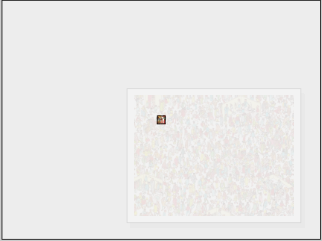
\includegraphics[width=.8\textwidth]{waldo2.PNG}
\end{column} 

\end{columns}
\end{frame}

\begin{frame}{Εφαρμογές στην κρυπτογραφία}
\begin{itemize}
\item Σχήματα αυθεντικοποίησης αντί για passwords
\begin{itemize}
\item Αντί για κωδικό: Απόδειξη ότι ο χρήστης τον γνωρίζει
\item Αποφεύγεται η μετάδοση και η επεξεργασία
\end{itemize}
\pause
\item Απόδειξη ότι το κρυπτοκείμενο περιέχει μήνυμα συγκεκριμένου τύπου
\pause
\item Ψηφιακές υπογραφές
\item Άντι-malleability
\pause 
\item Γενικά: Απόδειξη ότι παίκτης ακολουθεί κάποιο πρωτόκολλο χωρίς αποκάλυψη ιδιωτικών δεδομένων του
\end{itemize}
\end{frame}

\section{Συστήματα Αποδείξεων Μηδενικής Γνώσης}
\begin{frame}[allowframebreaks]{Διαλογικά Συστήματα Αποδείξεων}
\begin{block}{Συμβολισμός}
\begin{itemize}
\item Γλώσσα $ \mathcal{L} \in \mathtt{NP}$
\item Πολυωνυμική Mηχανή Turing $\mathcal{M}$
\item $x \in \mathcal{L} \Leftrightarrow \exists w \in \{0,1\}^{p(|x|)}: M(x,w) = 1$
\item Δύο PPT μηχανές Turing πολυωνυμικού χρόνου \prv, \ver
\item $<\mathcal{P}(x,w), \mathcal{V}(x)>$ είναι η αλληλεπίδραση μεταξύ  \prv, \ver με κοινή (δημόσια είσοδο) το $x$ και ιδιωτική είσοδο του \prv το $w$.
\item $out_\mathcal{V}{<\mathcal{P}(x,w), \mathcal{V}(x)>}$ η έξοδος του \ver στο τέλος του πρωτοκόλλου
\end{itemize}
\end{block}

\framebreak

\begin{block}{Παράδειγμα}
\begin{itemize}
\item $\mathcal{L}$ η γλώσσα του προβλήματος του διακριτού λογαρίθμου
\item $x$ ένα στιγμιότυπο του προβλήματος $x=<p,g: <g>= \mathbb{Z}_p^*, b  \in_R \mathbb{Z}_p^*>$
\item $w$ ο 'μάρτυρας', δηλ. $a: b = g^a$
\end{itemize}
\end{block}

\framebreak

Μία απόδειξη μηδενικής γνώσης για την $ \mathcal{L} $ είναι μία αλληλεπίδραση $<\mathcal{P}(x,w), \mathcal{V}(x)>$ με τις εξής ιδιότητες:

\begin{block}{\textbf{Πληρότητα - Completeness}}  
Ένας \emph{τίμιος} \prv, πείθει έναν \emph{τίμιο} \ver με  βεβαιότητα 

Αν  $x \in \mathcal{L}$ και $M(x,w) = 1$
\begin{align*}
Pr[out_{\mathcal{V}}<\mathcal{P}(x,w), \mathcal{V}(x)>(x)=1] = 1  
\end{align*}
\end{block} 

\framebreak

\begin{block}{\textbf{Ορθότητα - Soundness}}
Ένας \emph{κακόβουλος} $\mathcal{P}$ (σμβ. με $\mathcal{P}^*$), δεν μπορεί να πείσει \emph{τίμιο} \ver, παρά με αμελητέα πιθανότητα.

Αν $x \notin \mathcal{L}$ τότε $\forall (\mathcal{P}^*,w)$: 

\begin{align*}
Pr[out_{\mathcal{V}}<\mathcal{P}^*(x,w), \mathcal{V}(x)>(x)=1] = negl(\lambda)
\end{align*} 
\end{block}

\textbf{Παρατήρηση: }\\
Proof of Knowledge: O $\mathcal{P}^*$ \alert{δεν} είναι PPT. \\
Argument of Knowledge: O $\mathcal{P}^*$  είναι PPT.

\framebreak

\begin{block}{\textbf{(Τέλεια) Μηδενική Γνώση:}}
O \ver δεν μαθαίνει τίποτε εκτός, από το γεγονός ότι ο ισχυρισμός του \prv είναι αληθής.
 
\blue{Για κάθε PPT $\mathcal{V}^*$} \magenta{υπάρχει μία PPT \siml}: 

Αν  $x \in \mathcal{L}$ και $M(x,w) = 1$ οι τυχαίες μεταβλητές 

$ out_{\mathcal{V}^*}<\mathcal{P}(x,w), \mathcal{V}^*(x)>(x) $ και 

$ out_{\mathcal{V}^*}<\mathcal{S}(x), \mathcal{V}^*(x)>(x) $ 

ακολουθούν ακριβώς την ίδια κατανομή.
\end{block}

Επιτρέπουμε και \alert{κακόβουλο verifier} που δεν ακολουθεί το πρωτόκολλο και προσπαθεί να μάθει το $w$

\framebreak

\begin{block}{Διαίσθηση}
Ό,τι μπορεί να υπολογίσει ο \ver μετά την συζήτηση με τον \prv, μπορεί να το υπολογίσει και με τον \siml (δηλαδή ουσιαστικά χωρίς τη συζήτηση
με τον \prv)

Άρα: η συζήτηση προσθέτει \emph{μηδενική γνώση}

\end{block}
\end{frame}

\begin{frame}{Απόδειξη ιδιότητας ΖΚ: Ο simulator}
{Θεωρητική κατασκευή με πρακτικές εφαρμογές}
\textbf{Δεν διαθέτει τον witness}
\pause
\begin{small}
\begin{itemize}
\setlength\itemsep{0.01em}
\item Προσομοίωση απόδειξης στη θέση του \prv
\item Αλληλεπιδρά με τον \ver
\pause
\item Δεν μπορούμε να ξεχωρίσουμε τις αλληλεπιδράσεις <\siml,\ver> και <\prv,\ver>
\pause
\item Επιτρέπουμε και rewinds:
\pause
\item Αν κάποια στιγμή ο \ver 'ρωτήσει' κάτι που δεν μπορεί να απαντήσει ο \siml τότε stop - rewind
\pause
\item Μηδενική γνώση αν ο \ver κάποια στιγμή αποδεχτεί (έστω και με rewinds)
\pause
\item Γιατί: \pause
Δεν μπορεί να ξεχωρίσει τον \prv (που διαθέτει witness) από τον \siml (που δεν διαθέτει) 
\pause
\item \green{Αρκεί ο \siml να παραμείνει PPT}
\pause
\item Συγκεκριμένα: Ένας \ver που εξάγει πληροφορία από τον \prv θα εξάγει την ίδια πληροφορία και από τον \siml (όπου δεν υπάρχει κάτι να εξαχθεί)

\end{itemize}
\end{small}
\end{frame}

\begin{frame}{Σχέση Oρθότητας - Μηδενικής Γνώσης}
\begin{itemize}
\item O \siml μοιάζει με κακό $\mathcal{P}^*$ (και οι δύο δεν διαθέτουν τον witness).
\item  Όμως: Ο \siml πρέπει να παραμείνει PPT, ενώ $\mathcal{P}^*$ όχι 
\item Για τον \prv
\begin{itemize}
\item Μηδενική γνώση στην περίπτωση που είναι γνωστός ο $w$
\item Ορθότητα στην περίπτωση που δεν είναι γνωστός ο $w$
\end{itemize}
\item Για τον \ver
\begin{itemize}
\item Στην ορθότητα πρέπει να είναι τίμιος
\item Στην μηδενική γνώση όχι
\end{itemize}

\end{itemize}
\end{frame}

\begin{frame}[allowframebreaks]{Παραλλαγές Μηδενικής Γνώσης}
\begin{itemize}
	\item \textbf{Black-Box Zero Knowledge} 
	
	\magenta{$\exists$ PPT \siml} , \blue{$\forall \mathcal{V}^*$}  \\
	$ out_{\mathcal{V}^*}<\mathcal{P}(x,w), \mathcal{V}^*(x)>(x) $ και $ out_{\mathcal{V}^*}<\mathcal{S}^{ \mathcal{V}^*}(x), \mathcal{V}^*(x)>(x) $ να ακολουθούν ακριβώς την ίδια κατανομή.
	
	Παρατηρήσεις: O \siml 
	\begin{itemize}
	    \item ισχύει για όλους τους \ver
	    \item έχει oracle access στον \ver
	    \item δηλ. ελέγχει το input, rewind αλλά όχι το output 
	\end{itemize}
	
	\framebreak
	
	\item \textbf{Statistical Zero Knowledge} Οι κατανομές των συζητήσεων με $\mathcal{P},\mathcal{S}$ έχουν αμελητέα στατιστική απόσταση. 
	$\Delta(X,Y) = \frac{1}{2} \sum_{u \in V}|Prob_[X=u] - Prov[Y=u]|=negl(\lambda)$
	
 	\item \textbf{Computational Zero Knowledge} Οι κατανομές των συζητήσεων με $\mathcal{P},\mathcal{S}$  δεν μπορούν να διαχωριστούν από κάποιον αντίπαλο με πολυωνυμική υπολογιστή ισχύ.
 	
	\framebreak
	
	\item \textbf{Honest Verifier Zero Knowledge}
	\begin{itemize}
	\item Ο \ver  είναι τίμιος δηλ:
	\item ακολουθεί το πρωτόκολλο
	\item τα μηνύματα του προέρχονται από την ομοιόμορφη κατανομή - δεν εξαρτώνται από τα μηνύματα του \prv 
	\item μοντελοποιεί και παθητικό αντίπαλο
	\end{itemize}	  
	Πρακτικά: ο \siml παράγει συζητήσεις οι οποίες έχουν ίδια κατανομή με αυθεντικές $<\mathcal{P}(x,w), \mathcal{V}(x)>$ 
\end{itemize}

\end{frame}

\begin{frame}{Διαφορά ZK - HVZK}
    \begin{block}{... είναι στον \ver}
    \begin{itemize}
        \item Σε HVZK:
        \begin{itemize}
            \item Τα μηνύματα του \ver είναι τυχαία 
            \item Μπορούν να προετοιμαστούν εκ των προτέρων  από τον \siml
            \item Άρα o \ver \emph{δεν χρειάζεται} (non interactive)
        \end{itemize} 
        \item Σε ZK:
        \begin{itemize}
            \item Τα μηνύματα του \ver εξαρτώνται από τα μηνύματα του \prv
        \end{itemize}
    \end{itemize}    
    \end{block}
\end{frame}

\begin{frame}{Παραλλαγές Ορθότητας}
\begin{block}{Ειδική ορθότητα (special soundness)}
Υπάρχει ένας PPT αλγόριθμος (extractor), $\mathcal{E}$ ο οποίος αν δεχθεί \emph{πολλά} transcripts του πρωτοκόλλου με το ίδιο αρχικό μήνυμα από τον \prv αλλά διαφορετικές προκλήσεις από τον \ver μπορεί να εξάγει τον witness.
\end{block}
\pause
\begin{block}{Θεώρημα}
Ειδική ορθότητα $\Rightarrow$ ορθότητα με πιθανότητα false-positive $\frac{1}{|C|}$ όπου:
$C$: το σύνολο προέλευσης των μηνυμάτων του \ver

Ειδική ορθότητα $\Rightarrow$ απόδειξη γνώσης
\end{block}


\end{frame}

\begin{frame}{3-colorability}
\begin{columns}
\column{0.5\textwidth}
\begin{center}
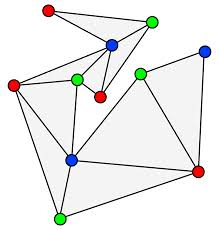
\includegraphics[scale=0.5]{3cp.jpg}
\end{center}

\column{0.5\textwidth}
\begin{block}{Ορισμός}
Γράφημα $G=(V,E)$ \\ \pause
O \prv  γνωρίζει ένα χρωματισμό  $c:V \rightarrow \{ 1,2,3 \}$  \\ \pause
Έγκυρος χρωματισμός: Γειτονικές κορυφές έχουν διαφορετικό χρώμα
$(v_i, v_j) \in E \Rightarrow   c(v_i) \neq c(v_j)$\\
\end{block}
\end{columns}
NP-Complete
\end{frame}
 
\begin{frame}{ZKP for 3-colorability}{Γενική Περιγραφή}
\begin{columns}
\column{0.73\textwidth}
\begin{small}
\begin{enumerate}
 	\setlength \itemsep{0.1em}
	\item \prv: επιλέγει μια τυχαία μετάθεση $\pi$ του $\{ 1,2,3 \}$. \pause
	\begin{itemize}
		\item Προκύπτει εναλλακτικός έγκυρος 3 - χρωματισμός $\pi.c$ του $G$. \pause
		\item Χρήση σχήματος δέσμευσης για τον εναλλακτικό χρωματισμό
		\item Yπολογίζει $commit( (\pi.c)(v_i), r_i) \forall v_i \in V$ 
		\item Αποστολή στον \ver \pause
	\end{itemize}
	\item \ver: επιλέγει μία τυχαία ακμή $(v_i, v_j) \in E$ και την στέλνει στον \prv. \pause
	\item \prv: ανοίγει τις δεσμεύσεις - αποκαλύπτει τις τιμές $\pi.c(v_i),\pi.c(v_j)$ και $r_i, r_j$ \pause
	\item \ver: ελέγχει αν $\pi.c(v_i) \neq \pi.c(v_j)$ και οι δεσμεύσεις είναι έγκυρες
	\item Επανάληψη
\end{enumerate}
\end{small}
\column{0.27\textwidth}
\begin{center}
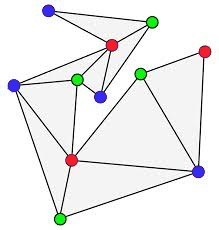
\includegraphics[scale=0.6]{3cp2.jpg}
\end{center}
\end{columns}
\end{frame}

 
\begin{frame}{ZKP for 3-colorability: Ιδιότητες (Πληρότητα)} 
\begin{itemize}
\item \textbf{Πληρότητα}\\
Αν ο $c$ είναι έγκυρος χρωματισμός τότε και ο $\pi.c$ είναι έγκυρος χρωματισμός.
\end{itemize}
\end{frame}


\begin{frame}{ZKP for 3-colorability: Ιδιότητες (Ορθότητα)} 
\begin{itemize}
\item \textbf{Ορθότητα}\\
Έστω $\mathcal{P}^*$ με μη έγκυρο χρωματισμό για κάποιο γράφημα:

Δηλ. \alert{τουλάχιστον 2 γειτονικές κορυφές με το ίδιο χρώμα}:
\pause

Πιθανότητα ανίχνευσης εξαπάτησης από \ver = Πιθανότητα επιλογής 'κακής' ακμής = $\frac{1}{|E|}$  \\

Πιθανότητα επιτυχούς εξαπάτησης από $\mathcal{P}^*$ = $1-\frac{1}{|E|}$
\pause

Σε $|E|^2$ επαναλήψεις και εφόσον
\begin{center}
$(1+\frac{t}{n})^n \leq e^t$
\end{center}

\medskip
Πιθανότητα επιτυχίας του  $\mathcal{P}^*$:

\begin{center}
$(1-\frac{1}{|E|})^{|E|^2} \leq e^{-|E|}$ \alert{αμελητέα} ως προς το μέγεθος του γραφήματος
\end{center}

\end{itemize}
\end{frame}

\begin{frame}{ZKP for 3-colorability: Ιδιότητες (Μηδενική Γνώση)} 
\begin{itemize}
\item \textbf{Μηδενική Γνώση} 
\begin{itemize}
\item Χρήση \siml χωρίς γνώση έγκυρου χρωματισμού - επιλογή τυχαίου

\item Πιθανότητα επιλογής από \ver ακμής με διαφορετικά χρώματα κορυφών $\frac{2}{3}$
\item Πιθανότητα επιλογής από \ver ακμής με ίδια χρώματα κορυφών  $\frac{1}{3}$
\item Αν ο \ver επιλέγει 'κακή' ακμή, rewind

\item Για $k$ επιτυχείς επιλογές χρειάζονται κατά μέσο όρο $2k$ εκτελέσεις

\end{itemize}
\end{itemize}
\pause
\begin{small}
Ο \siml δεν απαιτεί πολύ περισσότερο χρόνο από έναν \prv με γνώση του $c$

\alert{Όμως οι συζητήσεις δεν είναι πανομοιότυπες! (Γιατί;)}

\pause 
Τα commitments του \prv είναι έγκυροι χρωματισμοί, ενώ του \siml όχι!
\pause
\begin{block}{Συνέπεια [GMW91]}
Αν υπάρχουν μονόδρομες συναρτήσεις τότε όλο το NP έχει αποδείξεις μηδενικής γνώσης (black box computational)
\end{block}
\end{small}
\end{frame}



\section{Σ-πρωτόκολλα}

\begin{frame}{Σ-πρωτόκολλα}
Ένα πρωτόκολλο 3 γύρων με honest verifier και special soundness
\begin{enumerate}
	\item \textbf{Commit} O \prv δεσμεύεται σε μία τιμή.
	\item \textbf{Challenge} Ο \ver διαλέγει μία τυχαία πρόκληση. Εφόσον είναι τίμιος θεωρούμε ότι η πιθανότητα επιλογής πρόκλησης είναι ομοιόμορφα κατανεμημένη.
	\item \textbf{Response} O \prv απαντάει χρησιμοποιώντας τη δέσμευση, το μυστικό και την τυχαία τιμή. 
\end{enumerate}

\begin{block}{Special Soundness}
Δύο εκτελέσεις του πρωτοκόλλου με το ίδιο commitment, οδηγούν στην αποκάλυψη του witness
\end{block}
\end{frame}

\begin{frame}[allowframebreaks]{Γνώση DLOG:Το πρωτόκολλο του Schnorr}
\begin{block}{Γνωστά Στοιχεία}
\begin{itemize}
\item \textbf{Δημόσια:} Γεννήτορας $g$ μιας (υπό)ομάδας τάξης $q$ του $\zs{p}$ με δύσκολο DLP και στοιχείο $h \in \zs{p}$ 
\item \textbf{Ιδιωτικά:} O \prv έχει ένα witness $x \in \zs{q}$ ώστε $h = g^x \pmod{p}$
\end{itemize}
\end{block}

\begin{block}{Στόχος}
Απόδειξη κατοχής του $x$ χωρίς να αποκαλυφθεί.
\end{block}

\begin{block}{Συμβολισμός Camenisch-Stadler}
$PoK \{(x): g^x = h \pmod{p}, h,g \in_R \mathbb{Z}_p^* \}$ 
\end{block}

\framebreak
\begin{columns}
\column{0.5\textwidth}
\begin{small}
\begin{itemize}
\item  \textbf{Commit (\prv $\rightarrow$ \ver):} 
\begin{itemize}
\item Τυχαία επιλογή $t \in_R \zs{q}$ 
\item Yπολογισμός $y = g^t \bmod{p}$. 
\item Αποστολή $y$  στον \ver. 
\end{itemize}
\item \textbf{Challenge (\ver $\rightarrow$ \prv):} \\  Τυχαία επιλογή και αποστολή $c \in_R \zs{q}$
\item \textbf{Response (\prv $\rightarrow$ \ver):} \\   O \prv υπολογίζει το $s=t+cx \bmod{q}$ και το στέλνει στον \ver
\item  Ο \ver αποδέχεται αν\\ $g^s = yh^c \pmod{p}$
\end{itemize}
\end{small}
\column{0.5\textwidth}
\begin{figure}
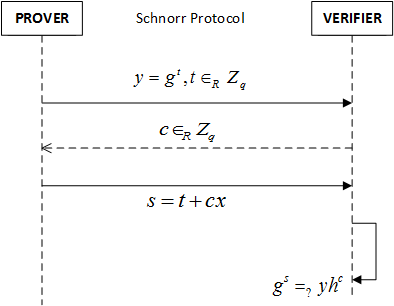
\includegraphics[width=1\textwidth]{schnorr.png}
\end{figure}
\end{columns}
\end{frame}

\begin{frame}{Πρωτόκολλο Schnorr: Πληρότητα}
 
\begin{itemize}
\item \textbf{Πληρότητα}\\

\pause
\begin{center}
$g^s = g^{t+cx} = g^t g^{cx} = yh^c \pmod{p}$
\end{center}



\end{itemize}
\end{frame}


\begin{frame}{Πρωτόκολλο Schnorr: Ορθότητα}
\begin{itemize}
\item \textbf{Ορθότητα} 
Πιθανότητα ο \prv$^*$ να ξεγελάσει τίμιο verifier: $\frac{1}{q}$ - αμελητέα - επανάληψη για μεγαλύτερη σιγουριά
\pause
\item \textbf{Special soundness}\\
Έστω 2 επιτυχείς εκτελέσεις του πρωτοκόλλου $(y,c,s)$ και $(y,c',s')$
\pause
\begin{align*}
 g^s = yh^c  \text{ και }  g^{s'} = yh^{c'}  \Rightarrow  g^s h^{-c}   = g^{s'} h^{-c'}  \Rightarrow \\
 g^{s-xc} = g^{s'-xc'} \Rightarrow  s-xc = s'-xc' \Rightarrow \\
 x = \frac{c'-c}{s-s}
\end{align*}
\pause
Αφού o \prv μπορεί να απαντήσει 2 τέτοιες ερωτήσεις ξέρει το DLOG
(ορθότητα και γνώση)
\end{itemize}
\end{frame}


\begin{frame}{Πρωτόκολλο Schnorr: HVZK}
\begin{itemize}
\item Διαθέτει \green{Honest Verifier Zero Knowledge}

Έστω  \siml που δεν γνωρίζει το $x$ και τίμιος \ver 
\pause
\begin{itemize}
\item Αρχικά o \siml δεσμεύεται κανονικά στο $y=g^t, t \in_R \zs{q}$
\pause
\item Ο \ver επιλέγει $c \in_R \zs{q}$
\pause
\item Αν ο \siml μπορεί να απαντήσει (αμελητέα πιθανότητα) το πρωτόκολλο συνεχίζει κανονικά \pause
\item Αλλιώς γίνεται rewind ο \ver (ίδιo random tape) \pause
\item Στη δεύτερη εκτέλεση \siml δεσμεύεται στο $y=g^t h^{-c}, t \in_R \zs{q}$ \pause
\item Ο \ver επιλέγει ίδιο $c \in_R \zs{q}$ (ίδιο random tape) \pause
\item O \siml στέλνει $s=t$ \pause
\item Ο \ver θα δεχτεί αφού \\
$yh^{c} = g^t  h^{-c} h^{c} = g^t = g^s$ \\
\end{itemize}
\end{itemize}
\pause
 
\begin{block}{Δηλαδή:}
Η συζήτηση $(t \in_R \mathbb{Z}_q; g^t h^{-c}   , c \in_R \mathbb{Z}_q  , t )$ 
 και η $(t,c \in_R \mathbb{Z}_q;  g^t  , c  , t+xc  )$
 ακολουθούν την ίδια κατανομή
 \end{block}
\end{frame}

\begin{frame}{Πρωτόκολλο Schnorr: ZK}

\textbf{Μηδενική Γνώση}: \alert{Δε διαθέτει}
\pause
\begin{itemize}
\item Ένας cheating verifier δε διαλέγει τυχαία \pause
\item Bασίζει κάθε challenge στο commitment που έλαβε πριν από τον \siml \pause
\item Στη simulated εκτέλεση δεν θα επιλέξει το ίδιο challenge \pause
\item Αμελητέα πιθανότητα να μπορεί να απαντηθεί από τον \siml \pause
\end{itemize}

Ενίσχυση για μηδενική γνώση: \pause

\begin{itemize}
\item Προσθήκη δέσμευσης από τον \ver στην τυχαιότητα \emph{πριν} το πρώτο μήνυμα του \prv ή \pause
\item Challenge space $\{ 0 , 1 \} $ (γιατί;) \pause
\item Ο \ver έχει δύο επιλογές μόνο για επιλογή πρόκλησης. 
\item Αν αλλάξει, ο \siml μπορεί να προετοιμαστεί και για τις δύο περιπτώσεις.
\end{itemize} 

\end{frame}

\begin{frame}[allowframebreaks]{Ισότητα DLOG:Το πρωτόκολλο Chaum Pedersen}
\begin{block}{Γνωστά Στοιχεία}
\begin{itemize}
\item \textbf{Δημόσια:} Γεννήτορες $g_1, g_2$ μιας (υπό)ομάδας τάξης $q$ του $\zs{p}$ με δύσκολο DLP και 2 στοιχεία $h_1, h_2 \in \zs{p}$ 
\item \textbf{Ιδιωτικά:} O \prv έχει ένα witness $x \in \mathbb{Z}_q$  ώστε $h_1 = g_{1}^{x} \bmod{p}$, $h_2 = g_{2}^{x} \bmod{p}$
\end{itemize}
\end{block}

\begin{block}{Στόχος}
Απόδειξη γνώσης του $x$ χωρίς να αποκαλυφθεί

Απόδειξη ισότητας διακριτών λογαρίθμων
\end{block}

\begin{small}
$PoK \{(x): h_1 = g_1^x \pmod{p} \wedge h_2 = g_2^x \pmod{p},  h_1,g_1,h_2,g_2 \in_R \mathbb{Z}_p^* \}$
\end{small}

\begin{columns}

\column{0.5\textwidth}
\begin{small}
\begin{itemize}
\item  \textbf{Commit:}
\begin{itemize}
\item Ο \prv  διαλέγει $t \in_R \mathbb{Z}_q$
\item Yπολογίζει $y_1 = g_{1}^{t} \bmod{p}$\\ $y_2 = g_{2}^{t} \bmod{p}$
\item Αποστέλλει $y_1, y_2$  στον \ver 
\end{itemize}
\item  \textbf{Challenge:}\\  
Ο \ver διαλέγει και αποστέλλει $c \in_R \mathbb{Z}_q$ 
\item  \textbf{Response:}\\   
Ο \prv υπολογίζει $s = t+cx \bmod{q}$ και το στέλνει στον \ver
\end{itemize} 
\end{small}
\column{0.5\textwidth}
\begin{figure}
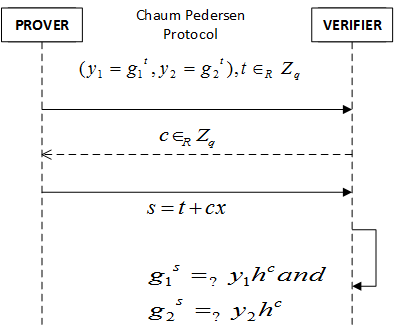
\includegraphics[width=1\textwidth]{chaumpedersen.png} 
\end{figure}
\end{columns}

\begin{center}
Ο \ver δέχεται αν  $g^s_1 = y_1h_{1}^c \pmod{p}$ και  $g^s_2 = y_2h_{2}^c \pmod{p}$ 
\end{center}


\end{frame}

\begin{frame}[allowframebreaks]{Ιδιότητες Chaum-Pedersen}
\begin{itemize}
\item \textbf{Πληρότητα}\\
Αν $h_1 = g_1^x$ και $h_2 = g_2^x$ τότε:
\begin{align*}
g_1^s = g_1^{t+xc} = y_1h_1^c \\
g_2^s = g_2^{t+xc} = y_2h_2^c
\end{align*}
\item \textbf{Special soundness}\\
Έστω δύο αποδεκτά transcripts με το ίδιο commitment $((y_1,y_2),c,s)$ και $((y_1,y_2),c',s')$
\begin{align*}
g_1^s =  y_1h_1^c \text{  και  } g_1^{s'} =  y_1h_1^{c'} \Rightarrow g_1^s h_1^{-c} = g_1^{s'} h_1^{-c'} \\
g_2^s =  y_2h_2^c \text{  και  } g_2^{s'} =  y_2h_2^{c'} \Rightarrow g_2^s h_2^{-c} = g_2^{s'} h_2^{-c'}
\end{align*}
Όπως σε Schnorr $x = \frac{s-s'}{c'-c}$
\framebreak
\item \textbf{Honest verifier zero knowledge}\\
Πραγματικό transcript με $c \in_R \mathbb{Z}_q$: 
\begin{center}
$(t \in_R \mathbb{Z}_q;(g_1^t,g_2^t), \quad c \in_R \mathbb{Z}_q,\quad t+xc \bmod{q})$
\end{center}
Simulated transcript με $c \in_R \mathbb{Z}_q$: 
\begin{center}
$(t,c \in_R \mathbb{Z}_q;(g_1^t h_1^{-c},g_2^th_2^{-c}), \quad c, \quad t)$
\end{center}
Ίδιες κατανομές αν $x=log_{g_1}{h_1}=log_{g_2}{h_2}$
\end{itemize}
\end{frame}

\begin{frame}{Εφαρμογές}
\begin{small}
\begin{block}{Έλεγχος για τριάδες DH}
Η τριάδα $(g^a,g^b,g^c)$ είναι τριάδα DH (δηλ. $g^c = g^{ab}$) 
\end{block}
\pause
Εκτελούμε $\mathtt{CH}(g_1 = g,g_2 = g^b,h_1 = g^a, h_2 = g^{ab} = {g^b}^a)$ με witness $a$
\begin{block}{Εγκυρότητα κρυπτογράφησης El-Gamal}
Δίνεται ένα ζεύγος στοιχείων του $\zs{p}$ τα $(c_1,c_2)$. 

Να δειχθεί ότι αποτελούν έγκυρη κρυπτογράφηση ενός μηνύματος $m$.
\end{block}
\pause
Αν είναι έγκυρη τότε πρέπει
\begin{align*}
(c_1,c_2) = (g^r, m \cdot h^r)
\end{align*}

Ισοδύναμα: 
\begin{align*}
log_g c_1 = log_h (\frac{c_2}{m}) 
\end{align*}
δηλ. ότι ο \prv είναι γνώστης της τυχαιότητας
\end{small} 
\end{frame}

\begin{frame}[allowframebreaks]{Σύνθεση $\Sigma$ πρωτοκόλλων}
\begin{block}{Θέωρημα} 
Τα $\Sigma$ πρωτόκολλα διατηρούν τις ιδιότητες τους αν συνδυαστούν με τις παρακάτω σχέσεις:
\end{block}
\begin{itemize}
\item $\mathtt{AND}$
\begin{itemize}
\item O \prv γνωρίζει 2 διαφορετικά $w$ για διαφορετικές σχέσεις.
\item Απόδειξη: 2 παράλληλες εκτελέσεις του  $\Sigma$ πρωτόκολλου με ίδιο challenge
\end{itemize}
\begin{figure}
\centering
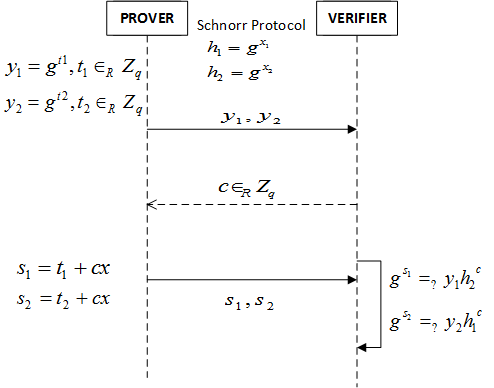
\includegraphics[width=0.6\textwidth]{schnorrand.png}
\end{figure}
\framebreak
\item Batch-AND\\
Μαζική επαλήθευση πολλαπλών σχέσεων με ένα πρωτόκολλο.
Για παράδειγμα: \\ 
$(g^a, g^b, g^{ab})$ ΚΑΙ  $(g^c, g^d, g^{cd})$ είναι τριάδες DH\\
Μπορώ να εκτελέσω το Chaum Pedersen για $(g^{ac}, g^{bd}, g^{abcd})$
\item $\mathtt{EQ}$
\begin{itemize}
\item O \prv γνωρίζει τον ίδιο $w$ για διαφορετικές σχέσεις.
\item Chaum Pedersen
\end{itemize}
\item $\mathtt{OR}$
\begin{itemize}
\item O \prv γνωρίζει \emph{κάποιο} $w$ για διαφορετικές σχέσεις.
\item Εφαρμογή: Απόδειξη ότι ο $w$ ανήκει σε ένα σύνολο
\end{itemize}
\end{itemize} 
\end{frame}

\begin{frame}{Γενικευμένη κατασκευή αποδείξεων OR}
\begin{itemize}
	\item Έστω $W = \{w_1, ..., w_n\}$ οι εναλλακτικοί μάρτυρες
	\pause
	\item Για αυτόν που κατέχει ο \prv ακολουθεί το πρωτόκολλο
	\pause
	\item Για τους υπόλοιπους ο \prv καλεί τον \siml ο οποίος υπολογίζει τις δεσμεύσεις που θα έκαναν τον \ver να δεχθεί σε μία προσομοιωμένη συζήτηση
	\pause
	\begin{itemize}
		\item \alert{Πρόβλημα:} O \siml δεν ξέρει το challenge
		\item \green{Λύση:} Το επιλέγει τυχαία
	\end{itemize} 
	\item Όλες οι δεσμεύσεις αποστέλλονται στον \ver 
	\pause
	\item Ο τελευταίος απαντάει με \emph{μία} τυχαία πρόκληση
	\pause
	\item O \prv ερμηνεύει την πρόκληση ως ένα μυστικό που πρέπει να χωριστεί
	\pause
	\item Κάθε μερίδιο θα χρησιμοποιείται στις απαντήσεις του \prv στο στάδιο Response
	\pause
	\item Ο \ver αποδέχεται αν όλες τις απαντήσεις που έλαβε στο τελευταίο βήμα είναι έγκυρες.
\end{itemize}
\end{frame}

\begin{frame}{OR-Schnorr}{$PoK \{(x_1,x_2): h_1 = g_1^{x_1} \pmod{p} \vee h_2 = g_2^{x_2} \pmod{p}$ \} }
Υποθέτουμε ότι ο \prv ξέρει το $x_1$
\begin{figure}
	\centering
	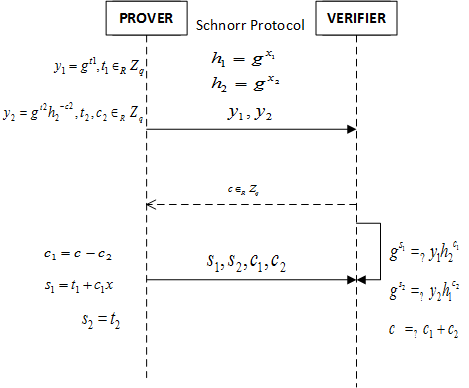
\includegraphics[width=0.8\textwidth]{schnorrwid.png}
\end{figure}
\end{frame}

%\begin{frame}{Γενίκευση}
%\setlength \itemsep{0.01pt}
%\begin{itemize}
%\item Γνώση $k$ από $n$ witnesses
%\item Χρήση $(n-k,n)$ threshold secret sharing
%\item Πώς:
%\begin{itemize}
%\item WLOG: Ο \prv δεν γνωρίζει τους $n-k$ πρώτους, γνωρίζει τους %υπόλοιπους $k$
%\item Commit: Επιλογή $n-k$ τιμών $c_i$ για χρήση στον \siml
%\item Challenge: O \ver στέλνει το $c$ (το μυστικό που πρέπει να %μοιραστεί)
%\item Response:
%\begin{itemize}
%\item Ο \prv επιλέγει βρίσκει πολυώνυμο $p$ που περνάει από τα %$\{(i, c_i)\}_{i=1}^{n-k} \cup (0,c)$
%\item Υπολογίζει τα $\{c_i = p(i) \}_{i=n-k+1}^n$ τα οποία %χρησιμοποιεί στο πρωτόκολλο
%\item Αποστέλει όλα τα $ \{ c_i, s_i \}_{i=1}^n$
%\item O \ver ελέγχει τις σχέσεις και αν μπορεί να γίνει η %ανακατασκευή του $c$
%\end{itemize} 
%\end{itemize}
%\end{itemize}
%\textbf{Επέκταση Σύνθεσης}: Για οποιοδήποτε σύνθετη μονότονη λογική %πρόταση (AND,OR)
%\end{frame}

\begin{frame}{Μη διαλογικές αποδείξεις}
\begin{block}{Ερώτηση}
Μπορούμε να καταργήσουμε τον \ver ;
\end{block}

O \prv παράγει την απόδειξη μόνος του

Η απόδειξη είναι επαληθεύσιμη από οποιονδήποτε

\begin{block}{Μετασχηματισμός: Fiat Shamir}
Αντικατάσταση της τυχαίας πρόκλησης με το αποτέλεσμα μιας ψευδοτυχαίας συνάρτησης με είσοδο τη δέσμευση (τουλάχιστον)

Συνήθως συνάρτηση σύνοψης - $\mathcal{H}$
\end{block}
\end{frame}

\begin{frame}{Non-interactive Schnorr}
\begin{block}{Γνωστά Στοιχεία}
\begin{itemize}
\item \textbf{Δημόσια:} Γεννήτορας $g$ μιας (υπό)ομάδας τάξης $q$ του $\zs{p}$ με δύσκολο DLP και στοιχείο $h \in \zs{p}$ 
\item \textbf{Ιδιωτικά:} O \prv έχει ένα witness $x \in \zs{q}$ ώστε $h = g^x \bmod{p}$
\end{itemize}
\end{block}
\pause
O  \prv:
\begin{itemize}
\item Τυχαία επιλογή $t \in_R \mathbb{Z}_{q}$,
\pause
\item Yπολογισμός $y = g^t \bmod{p}$
\pause
\item Υπολογισμός $c = \mathcal{H}(y)$ όπου $\mathcal{H}$ είναι μια συνάρτηση σύνοψης που δίνει τιμές στο $\mathbb{Z}_{q}$
\pause

\item Υπολογισμός $s=t+cx \bmod{q}$
\pause
\item Δημοσιοποίηση του $(h,c,s)$
\pause
\item Επαλήθευση (από οποιονδήποτε) $c = \mathcal{H} (g^s h^{-c})$
\end{itemize}
\end{frame} 

\begin{frame}[allowframebreaks]{Schnorr Signatures}

\textbf{Δημιουργία Κλειδιών:}
\begin{itemize}  
\item Επιλογή πρώτων $p,q$ ώστε το DLP
\item Επιλογή γεννήτορα $g$ σε υποομάδα του $\zs{p}$ με δύσκολο DLP
\item Επιλογή $x \in  \mathbb{Z}_q$ και υπολογισμός του $h = g^x \bmod{p}$
\item Δημόσιο κλειδί $(p,g,h)$, ιδιωτικό κλειδί $x$.
\end{itemize}

\framebreak

\textbf{Υπογραφή Μηνύματος $m$}
\begin{itemize}
\item Επιλογή τυχαίου $t \in \mathbb{Z}_q$
\item Υπολογισμός 
\begin{align*}
y  =   g^t \bmod p \textrm{ - δέσμευση}  \\
c  = \mathcal{H}(y,m) \textrm{ - υπογραφή εξαρτάται και από το μήνυμα} \\
s = t-cx \bmod{q}  \textrm{ - (για να μην χρειάζεται εύρεση αντιστρόφου)}
\end{align*} 
\item Υπογραφή είναι:$(c,s)$
\end{itemize}

\framebreak

\textbf{Επαλήθευση υπογραφής στο $m$}
\begin{align*}
\verify(h,m,(c,s)) =\twopartdef{1}{ c  = \mathcal{H}(g^s h^{c},m)  }{0}{\text{αλλιώς}} 
\end{align*}

\end{frame}
 
\section{Πηγές}
\begin{frame}[allowframebreaks]{Βιβλιογραφία}
\begin{tiny}
\begin{enumerate}
\item St. Zachos and Aris Pagourtzis. Στοιχεία Θεωρίας Αριθμών και Εφαρμογές στην Κρυπτογραφία. Πανεπιστημιακές Σημειώσεις
\item Jonathan Katz and Yehuda Lindell. Introduction to Modern Cryptography (Chapman and Hall/Crc Cryptography and Network Security Series). Chapman
and Hall/CRC, 2007
\item Paar, Christof, and Jan Pelzl. Understanding cryptography: a textbook for students and practitioners. Springer Science-Business Media, 2009.
\item Kiayias, Aggelos  \href{http://crypto.di.uoa.gr/class/Kryptographia/Semeioseis_files/Cryptograph_Primitives_and_Protocols.pdf}{Cryptography primitives and protocols}, UoA, 2015
\item \href{http://goo.gl/b75I29}{Nigel Smart. Introduction to cryptography}
\item Berry Schoenmakers. \href{http://www.win.tue.nl/~berry/2WC13/}{Cryptographic protocols}, 2015. 
\medskip
\item  D. Chaum and T. P. Pedersen. Wallet databases with observers. In Proceedings of the 12th Annual International Cryptology Conference on Advances in Cryptology, CRYPTO ’92, pages 89–105, London, UK, UK,1993. Springer-Verlag.
\item R. Cramer, I. Damgard, and B. Schoenmakers. Proofs of partial knowledge and simplified design of witness hiding protocols. In Proceedings of the 14th Annual International Cryptology Conference on Advances in Cryptology, CRYPTO ’94, pages 174–187, London, UK, UK, 1994. Springer-Verlag
\item A. Fiat and A. Shamir. How to prove yourself: practical solutions to identification and signature problems. In Proceedings on Advances in cryptology—CRYPTO ’86, pages 186–194, London, UK, UK, 1987. Springer-Verlag
\item O.Goldreich,S.Micali, and A.Wigderson. Proofs that yield nothing but their validity or all languages in np have zero-knowledge proof systems. J. ACM, 38(3):690–728, July 1991.
\item S Goldwasser, S Micali, and C Rackoff. The knowledge complexity of interactive proof-systems. In Proceedings of the seventeenth annual ACM symposium on Theory of computing, STOC ’85, pages 291–304, New York, NY, USA, 1985. ACM
\item  Jean-Jacques Quisquater, Louis Guillou, Marie Annick, and Tom Berson. 1989. \href{http://pages.cs.wisc.edu/~mkowalcz/628.pdf}{How to explain zero-knowledge protocols to your children}. In Proceedings on Advances in cryptology (CRYPTO '89), Gilles Brassard (Ed.). Springer-Verlag New York, Inc., New York, NY, USA, 628-631.  
\item Mike Rosulek, \href{http://web.engr.oregonstate.edu/~rosulekm/pubs/zk-waldo-talk.pdf}{Zero-Knoweldge Proofs, with applications to Sudoku and Where’s Waldo}
\item  C.P. Schnorr. Efficient signature generation by smart cards. Journal of Cryptology, 4(3):161–174, 1991
\item Online Lectures by \href{http://www.cs.jhu.edu/~susan/600.641/}{Susan Hohenberger},  \href{http://www.cs.cornell.edu/courses/cs6830/2014fa/}{Rafael Pass}
\item  Matthew Green, \href{http://blog.cryptographyengineering.com/2014/11/zero-knowledge-proofs-illustrated-primer.html}{Zero knowledge proofs: An illustrated primer}
\item Jeremy Kuhn \href{https://jeremykun.com/2016/07/05/zero-knowledge-proofs-a-primer/}{Zero Knowledge Proofs — A Primer}
\end{enumerate}
\end{tiny}
\end{frame}

\end{document}
